\documentclass[12pt]{article}
\usepackage[margin=3cm]{geometry}
\usepackage{graphicx}
\usepackage{float}
\usepackage{url}

\begin{document}

\begin{titlepage}
	\begin{center}
		
		
		% Upper part of the page. The '~' is needed because \\
		% only works if a paragraph has started.
		\vfill
		
		\textsc{\LARGE Lab 3: Inverter Layout}\\[1.5cm]
		
		\Large Adam Sumner\\[0.5cm]
		
		\Large Illinois Insititute of Technology\\[0.5cm]
		
		\Large ECE 429-01\\[0.5cm]	
		
		\noindent
		\vfill
		\large \textbf{Lab Date:} September 21\textsuperscript{st}, 2015\hfill
		\large \textbf{Due Date:} October 5\textsuperscript{th}, 2015
		% Bottom of the page
	
		
	\end{center}
\end{titlepage}

\section{Introduction}
The purpose of this experiment is to design the physical layout of an inverter using the Cadence Virtuoso Platform. The objectives are to implement the inverter layout design following industry standard design rules, and to validate the design using simulation software.
\section{Theory/Pre-Lab}
\subsection{Theory}
Layout design is often referred to as the ``Grunt work" of VLSI design. Regardless of its tedious nature, it is considered the most important part of the VLSI design process. This work is done through the use of a layout editor.

The underlying idea of a layout editor can be compared to a simple paint program, where individual pixels are modified. However, in a layout editor, the pixels are actually grid points, and ``paint operations" assign rectangular regions to layers that represent layout objects such as metal, polysilicon, contacts, etc. Using the FreePDK45 library, the minimum manufacturing grid is 2.5nm, however, this can require a lot of time fine tuning the design. While this size is preferred by experienced layout designers, this lab will use a minimum size of 10nm, since wasting small amounts of silicon area is not of this lab's concern. 

The FreePDK45 library has a list of design rules that need to be followed to ensure a proper layout. They are listed here: \url{http://www.eda.ncsu.edu/wiki/FreePDK45}. Because they can be quite complex, it is a silly thing to memorize them. Instead, design rule checking is a common practice used in industry. By frequently using DRC, violations of these design rules can be detected early to make the process go as smoothly as possible.

Because Layout designs and Schematics are created separately, there is a need to be able to easily compare the two. Luckily, Calibre is prepared with this functionality known as Layout vs. Schematic (LVS). Calibre LVS extracts a SPICE netlist from both the layout and the schematic, and then they are compared to see if they have the same set of transistors/connections.

Once the comparison is complete and the famous smiley face has been generated (no errors), a simulation can be be run. Because all layout related parasistics can be considered in the simulation, this is a more accurate representation of the functionality of the circuit in the real world. 
\subsection{Pre-Lab}
The preliminary assignment was to learn about the twin-well process, to study the FreePDK design rules, and to familiarize ones self with Tutorial II: Inverter Layout. All of these tasks were completed successfully.
\section{Implementation}
\subsection{Schematics}
\begin{figure}[H]
\centering
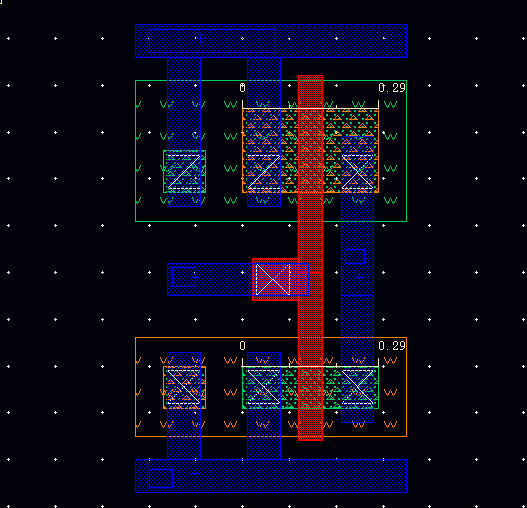
\includegraphics[width=1\linewidth]{layout}
\caption{Inverter Layout}
\label{fig:layout}
\end{figure}

\subsection{Procedure}
Due to the amount of tedious work involved in constructing the physical layout of the inverter, the details will not be shared explicitly. Please refer to Tutorial II: Inverter Layout for an in depth guide. The first part of the lab involved using Virtuoso to create the different layers of an inverter. This includes the p-well, n-well, well-tap, n-mos transistor, p-mos transistor, poly gate, vdd, gnd, input, output, and various metal connections. Throughout the design process, DRC was used to ensure the design rules were being followed. Once this was complete, the resulting schematic was created and is shown in Figure \ref{fig:layout}. Once finished, a DVL check was used to ensure that both the inverter schematic and the inverter layout were in accordance with each other. This is shown in Figure \ref{fig:lvs}. Finally once this was done, a SPICE netlist was generated from the layout and a simulation similar to Lab 2 was conducted. The results of $V_{in}$ vs $V_{out}$ are shown in Figure \ref{fig:graph}. 
\subsection{Results}
\begin{figure}[H]
\centering
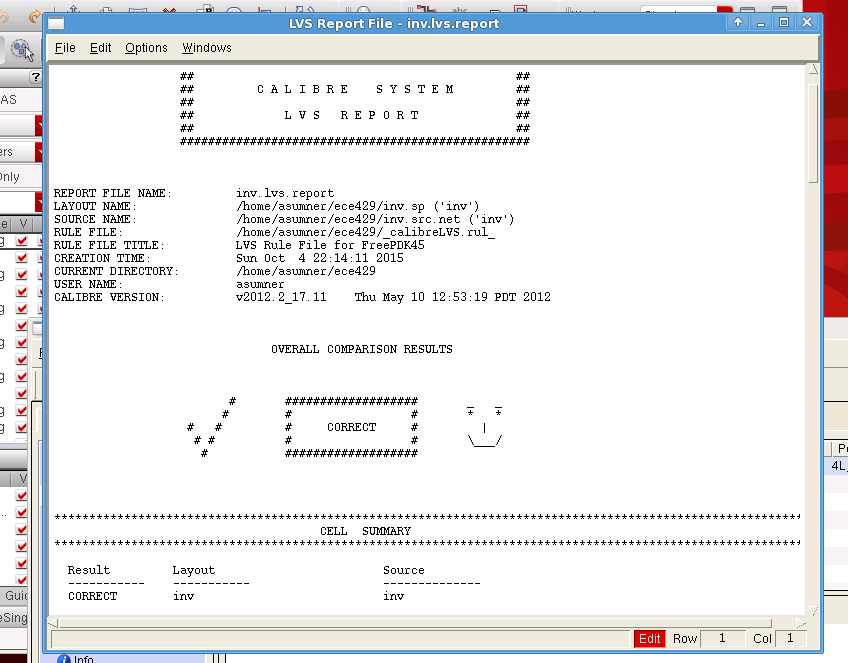
\includegraphics[width=1\linewidth]{lvs}
\caption{LVS Report (with smiley face)}
\label{fig:lvs}
\end{figure}

\begin{figure}[H]
\centering
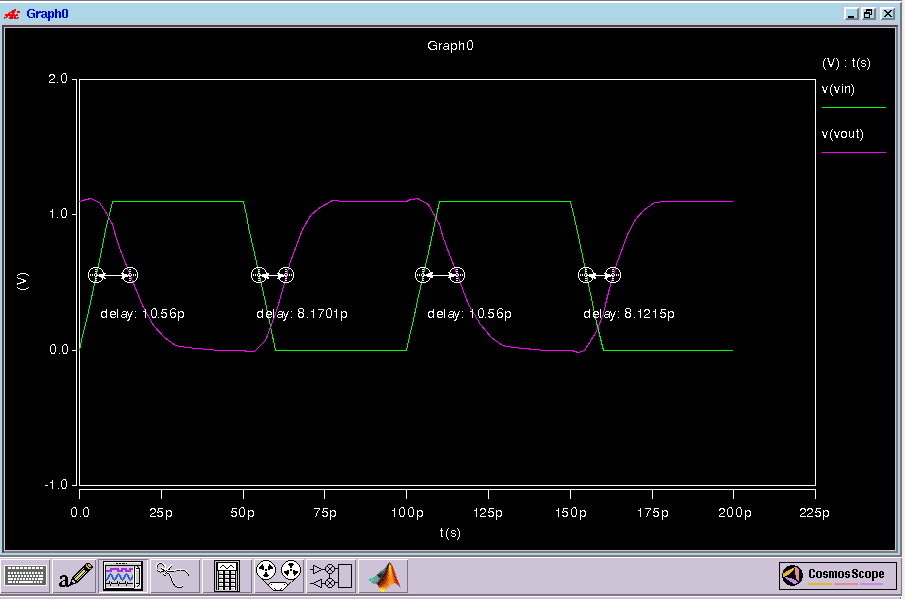
\includegraphics[width=1\linewidth]{graph}
\caption{Simulation Results}
\label{fig:graph}
\end{figure}



\subsection{Discussion}
Much like Lab 2, this experiment is designed to be an introduction lab. Its purpose is to teach the student how to work with the layout design mechanism of Virtuoso. Because of this, there is not much to be said about the data gathered other than the fact that it is indeed in accordance with the expected result and also matches the results obtained in Lab 2. It should be noted, however, that the time delay values of $V_{in}$ vs $V_{out}$ are larger than the time delay results from the schematic simulation. This is due to layout parasitic effects.
\subsection{Questions}
\begin{enumerate}
	\item \textbf{What determines the minimum transistor width and length for a specific technology?} \\
	A width rule and minimum channel length rule determine the width and length of a specific technology. These are both stated in the set of design rules chosen for the technology.
	\item \textbf{Why should well-taps connect to implanted regions instead of the wells directly?}\\
	The implant layer is what is used to form the well so it is necessary to connect the well-taps to this area.
	\item \textbf{What are the benefits of a twin-well process?} \\
	The benefits are that separate optimized wells can be achieved, and also balanced performance can be achieved for both n and p transistors
	\item \textbf{How do the delays of your inverter layout compare to that of the schematic in Lab 2? Do you expect them to be larger or smaller? Why?}\\
	The delays are longer than Lab 2. They are expected to be longer due to layout related parasitics. This is a more accurate simulation to represent an inverter produced in industry.
\end{enumerate}
%\subsection{Bonus Work}
\section{Conclusions}
Overall this experiment was a success. An inverter layout was designed, checked for design rule constraints, and simulated. The results obtained were in accordance with the expected result. This layout can be used for future experiments to gather accurate data.
\end{document}
